{\let\clearpage\relax\chapter*{Uzasadnienie wyboru tematu pracy}}
\addcontentsline{toc}{chapter}{Uzasadnienie wyboru tematu pracy}

Wraz z występującym w ostatnich latach systematycznym wzrostem liczby obrazowań medycznych uwidacznia się potrzeba na komputerowe wspomaganie pracy radiologów oceniających badania obrazowe. W szczególności zastosowanie znajdują aplikacje usprawniające generowanie raportów, rozwiązania do personalizacji diagnostyki i narzędzia poprawiające jej jakość.

Niniejsza praca, w odpowiedzi na powyższe zagadnienia, przedstawia propozycję strukturyzacji i automatyzacji oceny gojenia ścięgna Achillesa widocznego w obrazowaniu Rezonansem Magnetycznym (w skr. RM). Badanie to, w kontekście przedmiotowego ścięgna, jest dokładną metodą wykorzystywaną do oceny zmian strukturalnych i morfologicznych w zakresie tkanek miękkich. Wedle obecnych standardów ocena tego badania jest subiektywna i niesparametryzowana, a zatem stanowi ciekawy temat badawczy związany z możliwościami komputerowego wspomagania radiologów i usprawnienia ich pracy oraz w konsekwencji pomocy osobom ze schorzeniami ścięgna Achillesa.

Dodatkową motywację stanowi fakt dynamicznego rozwoju metod sztucznej inteligencji, a dokładniej ich podzbioru tj. głębokich sieci neuronowych, których rozwój znacząco przyspieszył od 2012 r. za sprawą innowacji w budowie sieci i szybkiej ewolucji możliwości sprzętowych. W szczególności konwolucyjne sieci neuronowe z uwagi na dużą skuteczność w problemach aplikowanych do przetwarzania obrazów znajdują zastosowanie w rosnącej liczbie narzędzi z certyfikacją medyczną dedykowanych dla radiologii.

Ograniczeniem wskazanych metod sztucznej inteligencji jest wymóg dużych, ustrukturyzowanych zbiorów danych, które mogą służyć do skutecznego uczenia się algorytmu. W toku prac nad wybraną problematyką, autor przedmiotowej rozprawy miał dostęp do unikatowego w skali światowej zbioru danych składającego się z 590 badań RM pacjentów po zerwaniu ścięgna Achillesa. Badania pochodziły z projektu START ("Wykorzystanie autologicznych mezenchymalnych komórek macierzystych w procesie regeneracji rekonstruowanego ścięgna Achillesa"), finansowanego przez Narodowe Centrum Badań i Rozwoju z krajowego programu STRATEGMED1.

Biorąc zatem pod uwagę występującą potrzebę w radiologii na wskazane innowacje, dynamiczny rozwój możliwości metod sztucznej inteligencji w tym zakresie i dostęp do zasobów umożliwiających realizację pierwszych w skali światowej badań nad możliwością strukturyzacji i automatyzacji oceny ścięgna Achillesa widocznego w badaniu RM, autor zdecydował się na wybór przedstawionej w pracy tematyki.  
 

{\let\clearpage\relax\chapter*{Cel i struktura pracy}}
\addcontentsline{toc}{chapter}{Cel i struktura pracy}

W ramach prac w projekcie START powstała koncepcja automatyzacji procesu monitorowania gojenia się ścięgna przy pomocy metod przetwarzania obrazów i sztucznej inteligencji. Założono, że głębokie sieci neuronowe będą skuteczne do oceny procesów patofizjologicznych widocznych w obrazowaniu medycznym takich jak gojenie tkanki miękkiej, co stanowi hipotezę przedmiotowej pracy.

Za cel główny autor postanowił obrać opracowanie automatycznej metody oceny gojenia się ścięgna Achillesa, natomiast cele poboczne stanowiły:
\begin{enumerate}[noitemsep,nolistsep]
	\item Wybór efektywnego kosztowo i czasowo protokołu badania bazującego na technikach obrazowania medycznego, a dokładniej Rezonansu Magnetycznego.
	\item Przetestowanie różnego rodzaju podejść związanych ze szkoleniem głębokich sieci neuronowych.
	\item Porównanie wyników oceny nowej metody z wynikami klasyfikacji bazującej na danych z ultrasonografii.
	\item Porównanie wyników oceny nowej metody z oceną funkcjonalną, rutynowo stosowaną do wspomagania rehabilitacji po urazie ścięgna.
\end{enumerate}

W celu uporządkowanego i zrozumiałego przedstawienia podłoża oraz wyników badań, w pracy wprowadzono podział na Rozdziały. Po wstępie i opisie celu pracy, w Rozdziale 3 zostały opisane współczesne metody monitorowania gojenia się ścięgna Achillesa. Rozdział ten rozpoczyna się od omówienia podstaw anatomicznych, biomechanicznych oraz dynamiki procesu gojenia się przedmiotowego ścięgna. Następnie przedstawiony jest szczegółowy opis badań obrazowych i biomechanicznych wykorzystywanych do oceny stanu rehabilitującego się pacjenta. 

W Rozdziale 4, omówione zostały szczegółowo konwolucyjne sieci neuronowe, które posłużyły jako rdzeń opracowanego rozwiązania. W szczególności, w opisie uwzględniono problemy z budową efektywnych modeli na bazie sieci neuronowych. 

W Rozdziale 5 zaprezentowano nowatorską metodę automatycznej oceny procesu gojenia się ścięgna Achillesa. Co istotne, omówiono unikatowy zbiór danych oraz wzorzec odniesienia, dzięki którym możliwa była realizacja przewidzianych badań i walidacja metody. Przedstawiono również eksperymenty wykorzystane do doboru komponentów i parametrów ostatecznego modelu oraz finalny wynik funkcjonowania opracowanego algorytmu. 

W Rozdziale 6 opisano zestawienie wyników metody z wynikami oceny realizowanej przez inne podejścia. W szczególności porównano przedmiotową metodę z metodą uczącą się explicite modelować ocenę radiologa, opracowaną również pod kierownictwem autora tej pracy w ramach pobocznych działań. Następnie zaprezentowano zestawienie z wynikami metody działającej w oparciu o dane z ultrasonografii, również opracowanej pod kierownictwem autora tej pracy. Finalnie, porównano wyniki z oceną biomechaniczną realizowaną standardowo przez fizjoterapeutów. Wnioski z porównań natury praktycznej spisano w Rozdziale 7. Całość pracy zakończono podsumowaniem przedstawionym w Rozdziale 8.

{\let\clearpage\relax\chapter*{Zbiór danych}}
\addcontentsline{toc}{chapter}{Zbiór danych}

W ramach projektu przebadano 59-ciu pacjentów po całkowitym zerwaniu ścięgna Achillesa i 27-ciu ochotników. Kryteria kwalifikacji i szczegóły dotyczące urazów opisano w pracy.

Podczas trwającej 12 miesięcy rehabilitacji pacjenci byli monitorowani z wykorzystaniem RM GE Signa HDxt 1.5T wyposażonego w cewkę Foot \& Ankle dedykowaną do pomiarów w rejonie dolnej kończyny. Każde z badań RM było wykonane z użyciem 7-miu sekwencji i łącznie 10-ciu modalności.

W grupie zdrowych ochotników przeprowadzono pojedyncze badanie, natomiast pacjentów skanowano 10-krotnie w odpowiednio zdefiniowanych odstępach czasowych. Pierwsze badanie odbyło się przed operacją, a następnych 9 odpowiednio w tygodniach: 1, 3, 6, 9, 12, 20, 26, 40 i 52 po operacji. Zbiory trójwymiarowe posłużyły do przygotowania dwuwymiarowych danych wejściowych dla wykorzystanych architektur sieci neuronowych. Finalna liczba tak utworzonych obrazów wyniosła 11.725 (oznaczonych jako obrazy zdrowego ścięgna) i 138.604 (oznaczonych jako obrazy chorego ścięgna). W zależności od wymogów eksperymentu liczby te były zmniejszane poprzez próbkowanie lub sztucznie powiększane z wykorzystaniem metod augmentacji danych.

Dodatkowo zgromadzono ustrukturyzowany opis radiologiczny dla 48-miu pacjentów w 10 krokach czasowych (480 ankiet z 6-cioma parametrami ocenionymi w skali 0--7). Czterech pacjentów (40 badań) zostało losowo wydzielonych na początku eksperymentów jako pacjenci testowi wykorzystani do celów wnioskowania i porównań wyników badań.

{\let\clearpage\relax\chapter*{Nowa metoda oceny ścięgna Achillesa}}
\addcontentsline{toc}{chapter}{Nowa metoda oceny ścięgna Achillesa}

W wyniku prac została opracowana komputerowa metoda oceny ścięgna Achillesa widocznego w badaniach RM, generująca numeryczny wynik w skali 0--7 dla 6-ciu zdefiniowanych w ramach projektu START radiologicznych parametrów opisujących strukturę i morfologię tkanek miękkich. Schemat generacji wartości pojedynczego parametru ilustruje rysunek poniżej. 
\begin{figure}[h!]
	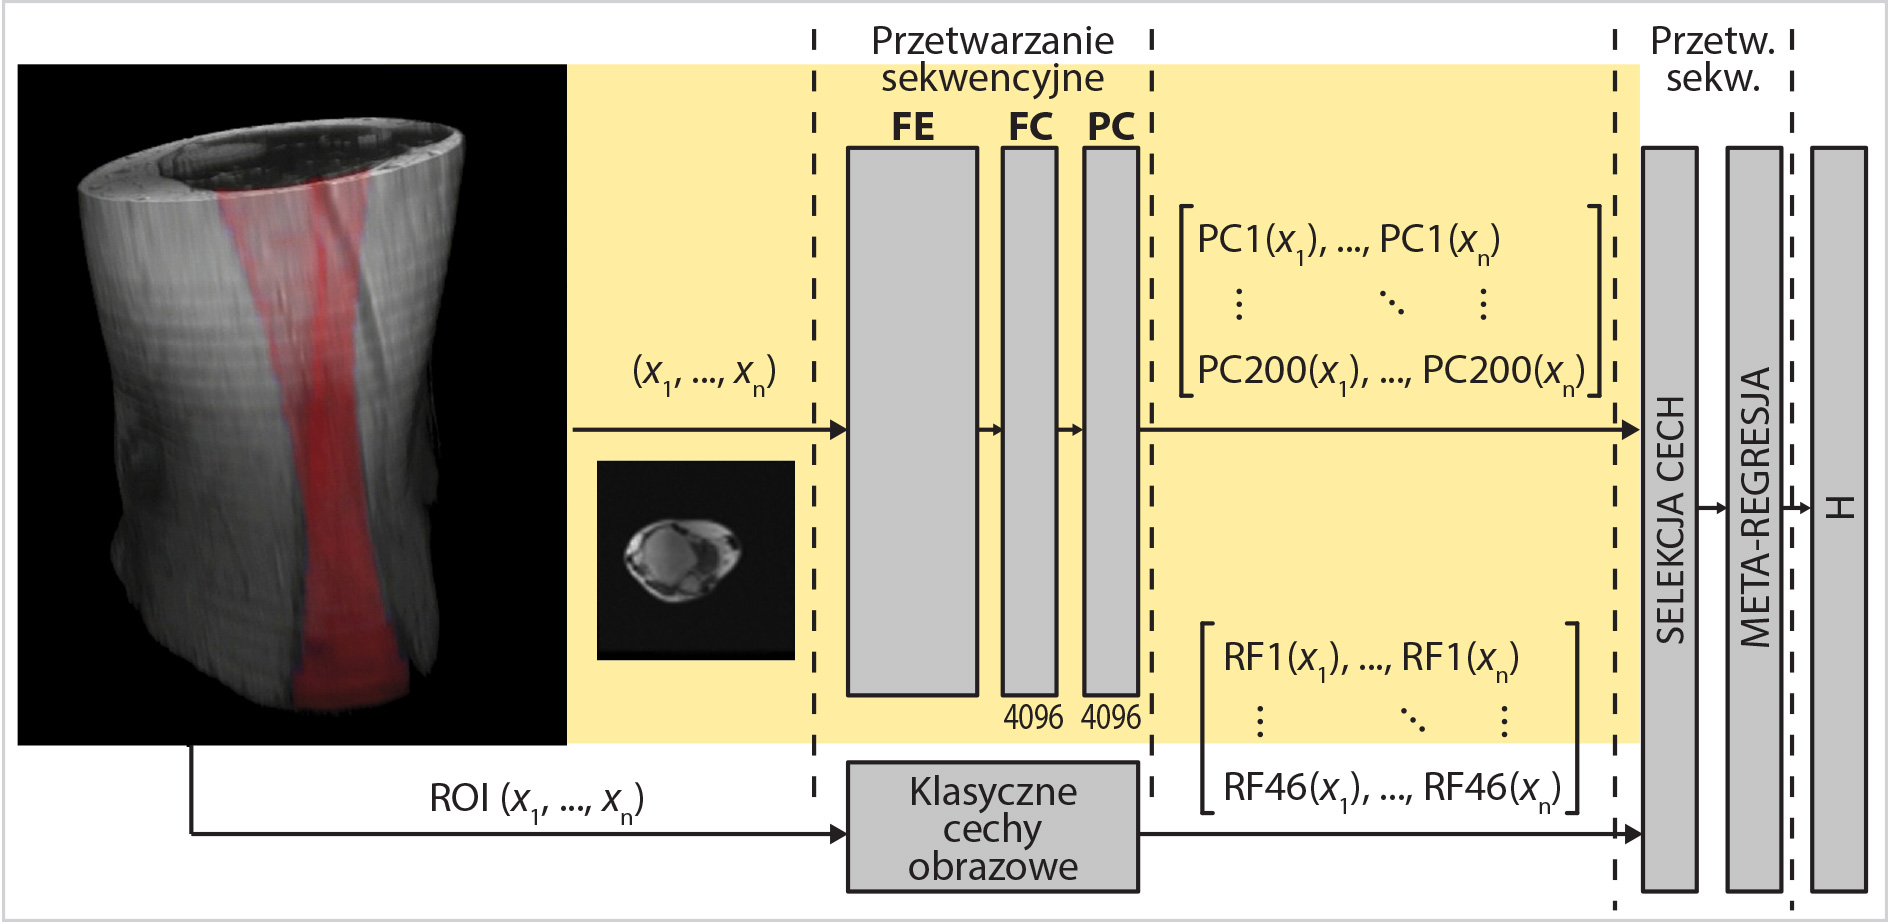
\includegraphics[width=\textwidth]{figures/net.jpg}
	\caption{Schemat automatycznej metody oceny pojedynczego parametru procesu gojenia się ścięgna Achillesa.} \label{fig:net}
\end{figure}

Dane wejściowe stanowi trójwymiarowe badanie RM obszaru podudzia. Badanie dzielone jest na $n$ obrazów będących przekrojami poprzecznymi względem osi długiej ścięgna. Z każdego przekroju dwojako ekstrahowane są zestawy cech. Po pierwsze, wykorzystywany jest ekstraktor cech będący zestawem warstw konwolucyjnych i jednej warstwy gęstej odpowiednio wytrenowanej sieci neuronowej na wyjściu (po redukcji z wykorzystaniem metody analizy czynników głównych) generującej 200 wartości. Po drugie, dla obszaru ścięgna widocznego na każdym z przekrojów, wyliczane są cechy statystyczne i teksturalne, których łączna liczba wynosi 46. Z pośród tak utworzonego zestawu 246 wartości, dla każdego z 6-ciu radiologicznych parametrów, wybierane są z wykorzystaniem metody LASSO optymalne podzbiory o liczebności mniejszej niż 20. Podzbiory są kolejno procesowane z wykorzystaniem regresji opartej o algorytm wektorów nośnych, której wyniki dla poszczególnych przekrojów łączone są z wykorzystaniem średniej trymowanej, odrzucając rezultaty skrajne i generując pojedynczą wartość parametru dla całego badania 3D RM.   


{\let\clearpage\relax\chapter*{Charakterystyka i wyniki przeprowadzonych badań}}
\addcontentsline{toc}{chapter}{Charakterystyka i wyniki przeprowadzonych badań}

-- wybór danych wejściowych
-- dobór parametrów FE
-- dobór parametrów PCA
-- dobór LASSO
-- wyniki, krzywe gojenia, ocena zbiorcza
-- porównanie z end-to-end, USG, biomechanika

{\let\clearpage\relax\chapter*{Wnioski końcowe}}
\addcontentsline{toc}{chapter}{Wnioski końcowe}

-- Wnioski
